\documentclass[12pt]{book}
\usepackage{hyperref}

\title{Physics of Complex Systems} \author{\url{https://github.com/Grufoony/Physics_Unibo}}
\date{}

\usepackage{amsmath}
\usepackage{amsfonts}
\usepackage{amssymb}
\usepackage{amsthm}
\usepackage{braket}
\usepackage[margin=3cm]{geometry}
\usepackage{pgfplots}
\pgfplotsset{compat=1.18}
\usepackage{fancyhdr}
\usepackage{physics}
\usepackage{systeme,mathtools}
\usepackage{graphicx}
\usepackage{float}
\usepackage{relsize}
\usepackage{calligra}
\usepackage{siunitx}
\usepackage{circuitikz}
\usepackage[miktex]{gnuplottex}
\usepackage{epstopdf}
\usepackage[english]{babel}
\usepackage{float}
\usepackage{tikz}


\newcommand{\vv}{\vec{v}}
\newcommand{\vw}{\vec{w}}
\newcommand{\vo}{\vec{0}}
\newcommand{\vx}{\vec{x}}
\newcommand{\R}{\Re}
\newcommand{\la}{\lambda}
\newcommand{\bd}{\textbf}
\newcommand{\lang}{\left\langle}
\newcommand{\rang}{\right\rangle}
\newcommand{\lbra}{\left\lbrace}
\newcommand{\rbra}{\right\rbrace}
\newcommand{\ih}{\hat{i}}
\newcommand{\jh}{\hat{j}}
\newcommand{\kh}{\hat{k}}
\newcommand{\vr}{\vec{r}}

\begin{document}

\maketitle
\tableofcontents
\pagebreak

\chapter{Introduction to Complex Systems}
Complex systems are interdisciplinary: you have to communicate your results to experts from different science field.
You need to provide an easy answer to a complex problem, no matter how difficult it's to get this answer.
\section{Emergence}
One of the main ideas in complex systems is emergence. Emergence means that the structure of the particles is simple and they are not so important like interactions bettween them. \\
An example of this is the Central limit theorem, which comes from mathematics. \\ \\
If you have a random variable $x_k$, with average value $\lang x_k \rang = 0$ and finite variance $\sigma^2$, then the central limit theorem says that, if the variables are independent (and in physics this is usally a fair assumption) for every value of $k$, then the normalized sum 
$$
	z_n = \frac{1}{\sqrt{N}}\sum_{k=0}^N x_k
$$
then the distribution of this variable $z_n$ is known, and it is gaussian, for a big enough value of $N$.
$$
	\rho(z_n) \sim \exp\left(-\frac{z^2}{2\sigma^2}\right)
$$
Despite the fact that we, as humans, need a cause-effect relationship to describe a phenomenon, nature loves independent events, like DNA mutations.
The gaussian describes the fluctuations of a system at equilibrium, not the complexity. You cannot extract work from fluctuations at equilibrium, otherwise you violate thermodynamics (and that's no good). \\
The gaussian function is not a physical function, because it implies non zero probabilities to events which are impossible. For example, if we take a particle in a basin of attraction of a potential, the non zero probability given by the gaussian fluctuations allows the particle to jump out of the pit. But this violates the second law of thermodynamics. \\ \\
A way to defy the gaussian properties is to allow a system to have memory, so to remove the independence of the variable. 
\begin{center}
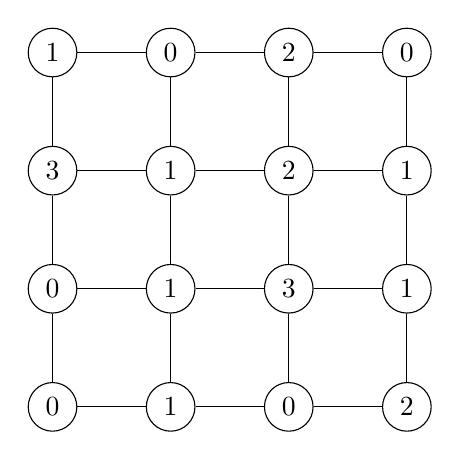
\begin{tikzpicture}[node distance={15mm}, main/.style = {draw,circle}]
\node[main] (1) {1};
\node[main] (2) [right of=1] {0};
\node[main] (3) [right of=2] {2};
\node[main] (4) [right of =3] {0};
\node[main] (5) [below of =1] {3};
\node[main] (6) [right of=5] {1};
\node[main] (7) [right of=6] {2};
\node[main] (8) [right of=7] {1};
\node[main] (9) [below of=5] {0};
\node[main] (10) [right of=9] {1};
\node[main] (11) [right of=10] {3};
\node[main] (12) [right of=11] {1};
\node[main] (13) [below of=9] {0};
\node[main] (14) [right of=13] {1};
\node[main] (15) [right of=14] {0};
\node[main] (16) [right of=15] {2};
\draw (1) -- (2);
\draw (1) -- (5);
\draw (2) -- (3);
\draw (3) -- (4);
\draw (5) -- (6);
\draw (6) -- (7);
\draw (7) -- (8);
\draw (5) -- (9);
\draw (9) -- (10);
\draw (10) -- (11);
\draw (11) -- (12);
\draw (9) -- (13);
\draw (13) -- (14);
\draw (14) -- (15);
\draw (15) -- (16);
\draw (2) -- (6);
\draw (3) -- (7);
\draw (4) -- (8);
\draw (6) -- (10);
\draw (7) -- (11);
\draw (8) -- (12);
\draw (10) -- (14);
\draw (11) -- (15);
\draw (12) -- (16);
\end{tikzpicture}
\end{center}
One example of this is the sand pile model. You have a lattice, and each point is connected to its four neighbors. At this point one particle is put in a randomly chosen point. Each node can have four possible states, $0,1,2,3$, that is four possible numbers of particles. If a node reaches 4 particles, the 4 particles are distributed to the 4 neightbouring nodes.
\begin{center}
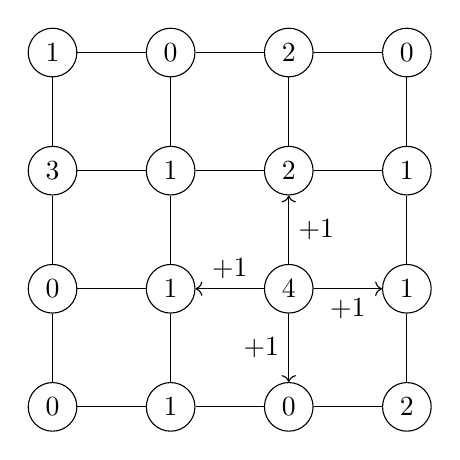
\begin{tikzpicture}[node distance={15mm}, main/.style = {draw,circle}]
\node[main] (1) {1};
\node[main] (2) [right of=1] {0};
\node[main] (3) [right of=2] {2};
\node[main] (4) [right of =3] {0};
\node[main] (5) [below of =1] {3};
\node[main] (6) [right of=5] {1};
\node[main] (7) [right of=6] {2};
\node[main] (8) [right of=7] {1};
\node[main] (9) [below of=5] {0};
\node[main] (10) [right of=9] {1};
\node[main] (11) [right of=10] {4};
\node[main] (12) [right of=11] {1};
\node[main] (13) [below of=9] {0};
\node[main] (14) [right of=13] {1};
\node[main] (15) [right of=14] {0};
\node[main] (16) [right of=15] {2};
\draw (1) -- (2);
\draw (1) -- (5);
\draw (2) -- (3);
\draw (3) -- (4);
\draw (5) -- (6);
\draw (6) -- (7);
\draw (7) -- (8);
\draw (5) -- (9);
\draw (9) -- (10);
\draw[->] (11) -- node[above]{+1} (10);
\draw[->] (11) -- node[below]{+1} (12);
\draw (9) -- (13);
\draw (13) -- (14);
\draw (14) -- (15);
\draw (15) -- (16);
\draw (2) -- (6);
\draw (3) -- (7);
\draw (4) -- (8);
\draw (6) -- (10);
\draw[->] (11) -- node[right]{+1} (7);
\draw (8) -- (12);
\draw (10) -- (14);
\draw[->] (11) -- node[left]{+1} (15);
\draw (12) -- (16);
\end{tikzpicture}
\end{center}
\begin{center}
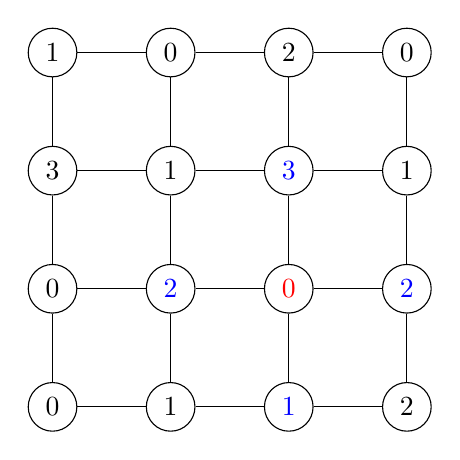
\begin{tikzpicture}[node distance={15mm}, main/.style = {draw,circle}]
\node[main] (1) {1};
\node[main] (2) [right of=1] {0};
\node[main] (3) [right of=2] {2};
\node[main] (4) [right of =3] {0};
\node[main] (5) [below of =1] {3};
\node[main] (6) [right of=5] {1};
\node[main] (7) [right of=6] {\textcolor{blue}{3}};
\node[main] (8) [right of=7] {1};
\node[main] (9) [below of=5] {0};
\node[main] (10) [right of=9] {\textcolor{blue}{2}};
\node[main] (11) [right of=10] {\textcolor{red}{0}};
\node[main] (12) [right of=11] {\textcolor{blue}{2}};
\node[main] (13) [below of=9] {0};
\node[main] (14) [right of=13] {1};
\node[main] (15) [right of=14] {\textcolor{blue}{1}};
\node[main] (16) [right of=15] {2};
\draw (1) -- (2);
\draw (1) -- (5);
\draw (2) -- (3);
\draw (3) -- (4);
\draw (5) -- (6);
\draw (6) -- (7);
\draw (7) -- (8);
\draw (5) -- (9);
\draw (9) -- (10);
\draw (11) -- (10);
\draw (11) -- (12);
\draw (9) -- (13);
\draw (13) -- (14);
\draw (14) -- (15);
\draw (15) -- (16);
\draw (2) -- (6);
\draw (3) -- (7);
\draw (4) -- (8);
\draw (6) -- (10);
\draw (11) -- (7);
\draw (8) -- (12);
\draw (10) -- (14);
\draw (11) --  (15);
\draw (12) -- (16);
\end{tikzpicture}
\end{center}
For the nodes in the border, what happens is that 2 of the particles are redistributed and the other 2 are released in the enviroment, so they are lost. \\ \\
So this system has memory, and this means that the states of all the nodes are not independent. This memory turns the gaussian distribution into a power law
$$
	p(n) \propto n^{-\alpha}
$$
with $\alpha > 1$. \\
The decay of the power low is much slower than that of the gaussian, which means that the probability to have events in the extremes is significantly higher with the power low distribution.
Memory is related to power laws, but vice versa is not guaranteed.
We can also have power laws in physics, for example in the Ising model.
In physics, power laws typically represent a phase transition for a dynamic system in a non-equilibrium state. \\
In the sand pile model, we notice a self-organized criticality: the system naturally goes into a critical state and does a phase transition. \\
Another example of a natural power law is the Kleiber law which relates the metabolic rate (amount of energy you need to survive) to the mass.
\begin{equation}
	E(m) \propto m^{\frac{4}{3}}
\end{equation}
We can also observe that heartbeat rate decreases with mass and lifetime increases.
\section{Network's energy}
Let's take a region of space containing a number $N$ of nodes. This system can represent, for example, the hydraulic network of a city. 
For a node we define its ``energy'' flow $\varphi$ (in the case of the hydraulic network, what is flowing between the nodes is water). How much ``energy'' do we need to insert in the system? \\
If we have to distribute something to all the nodes, the most basic way to do it is to connect one on one all the nodes, as to form a long chain. \\
\begin{center}
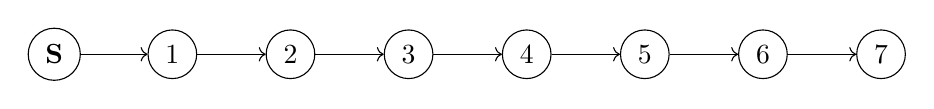
\begin{tikzpicture}[node distance={15mm}, main/.style = {draw,circle}]
\node[main] (1) {1};
\node[main] (0) [left of=1] {\textbf{S}};
\node[main] (2) [right of=1] {2};
\node[main] (3) [right of=2] {3};
\node[main] (4) [right of =3] {4};
\node[main] (5) [right of =4] {5};
\node[main] (6) [right of=5] {6};
\node[main] (7) [right of=6] {7};
\draw[->] (0) -- (1);
\draw[->] (1) -- (2);
\draw[->] (2) -- (3);
\draw[->] (3) -- (4);
\draw[->] (4) -- (5);
\draw[->] (5) -- (6);
\draw[->] (6) -- (7);
\end{tikzpicture}
\end{center}
If the flow out of the source $S$ is $\phi$, the flow after the first node is $\phi - \varphi$, and so on, and we expect that the flow arriving to the final node will be $\varphi$. \\
So the total energy is 
$$
	E_T \approx l\sum_{k=0}^{N-1} (\phi - k\varphi) = l\varphi\sum_{k=0}^{N-1} k`
$$
$$
	E_T \propto l\varphi N^2
$$
So the totaly energy that is required to provide for all the nodes, with this configuration, is proportional to the square of the total number of nodes. So with this configuration we have a network that is very easy to implement, but the network is very inefficient. \\ \\ 
Another possible connection of the nodes is the following one:
\begin{center}
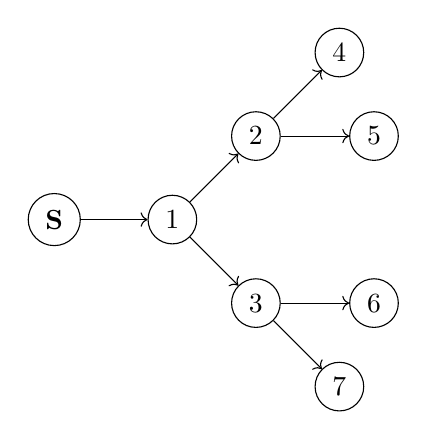
\begin{tikzpicture}[node distance={15mm}, main/.style = {draw,circle}]
\node[main] (1) {1};
\node[main] (0) [left of=1] {\textbf{S}};
\node[main] (2) [above right of=1] {2};
\node[main] (3) [below right of=1] {3};
\node[main] (4) [above right of =2] {4};
\node[main] (5) [right of =2] {5};
\node[main] (6) [right of=3] {6};
\node[main] (7) [below right of=3] {7};
\draw[->] (0) -- (1);
\draw[->] (1) -- (2);
\draw[->]  (1) -- (3);
\draw[->]  (2) -- (4);
\draw[->]  (2) -- (5);
\draw[->]  (3) -- (6);
\draw[->]  (3) -- (7);
\end{tikzpicture}
\end{center}
So each node is linked to two mode nodes. This is what is called a tree structure. \\
The main problem with such a structure is that the path between the nodes is always the same, but it is impossible to design a city in such a way. \\
The number of nodes is $N = 2^{m+1}$, where $m$ is the number of levels. \\
The relation for the flow in each level is
$$
	2\phi_k + \varphi = \phi_{k-1}
$$
where we assume again that the flow in the final level is $\varphi$. \\
$\phi_k$ then is
$$
	\phi_k = (2^{m+1-k}-1)\varphi
$$
Then:
$$
	E_T = d\varphi\sum_{k=1}^m 2^k(2^{m+1-k}-1) \approx d\varphi m 2^{m+1}	
$$
$$
	E_T = d\varphi N \log_2N
$$
This configuration is much more efficient than the previous alternative, although it is impossible to put to practice. \\ \\ 
So we need to find a solution that is in the middle of these two. \\ \\
Another possible structure consists of connecting all the nodes to the source, making a star network: also this model is of course impossible to put in practice. \\
However, in this case the total energy required is proportional to $NL$, where $L$ is the scale length of the system. 
$$
	E_T \propto NL
$$
The proportionality to $L$ is due to the fact that the average length of the links is proportional to the size of the space. \\
Since 
$$
	N = \left(\frac{L}{l} \right)^D
$$
where $D$ is the system dimension (e.g. 1D, 2D...).
We have that
$$
	E_T \propto N\overline{L} \approx N^{1+1/D} = V^{\frac{D+1}{D}}
$$
We notice that:
\begin{itemize}
	\item for a 2D system, like a city, $E \propto V^{\frac{3}{2}}$
	\item for a 3D system, like biological systems, $E \propto V^{\frac{4}{3}}$
\end{itemize}
In any case the exponent is greater than one so, soon or later, the system will collapse.
The problem is also logistic, because in a real transportation line there is also waste, that has to be disposed of. \\ \\
If we consider our system to be an animal's body, this would mean that in order to survive the amount of blood in its body must grow with the size by an amount of $4/3$. This would mean that very big animals can't survive, but they do, and the solution is in Kleiber's law. \\
As animals get bigger, their demand of energy goes down, so their metabolism slows down.  


Once we have a model (which hopefully is a good one), the model is deterministic, so if we know the initial conditions os the system, we know exactly what state the system will have at any future time. \\
The problem with this is that we don't know the initial conditions with absolute certainty. So at this point the question, that will be answered later, is: \\
How much error in the initial conditions is acceptable before that the previsions of our model start to diverge from the real evolution in an unacceptable way?
\section{Broken Stick Model}
Let's consider the portion $[0,1]$ of the axis, which represents a segment (a stick) of length 1. Suppose that we extract randomically a point $x_1$ on that segment, and we cut it in correspondence of that point, thus obtaining the portion $[0,x_1]$ of the axis. \\
By repeating this process many times, we obtain a system with memory, because of course the length of the segment at a certain iteration depends on all the previous iterations. \\
This is called the broken stick model. \\
For this system one expects to have a power law distribution, because if we rescale the variable $x$, the distribution must not change.
$$
	p(x) \sim \frac{1}{x^a}
$$
$$
	y = \la x \ \ \longrightarrow \ \ p(y) = \frac{1}{(\la x)^a} \sim \frac{1}{x^a}
$$
Since we have:
$$
	\lang x_k \rang = \frac{\lang x_{k-1} \rang}{2}
$$
$$
	\rho_N(2x) = \frac{1}{2}\rho_{N-1}(x)
$$
Which means that, as $N$ goes to infinity we get
$$
	\rho(2x) = \frac{1}{2}\rho(x)
$$
$$
	\rho(x) = \frac{1}{x}
$$
Let's now try to implement the system without memory. So we have $N$ independent variables $x_k$ uniformly distributed, and for each variable we define its distance from the previous one, $\Delta x$. \\
The probability to find $\Delta x$ is the probability of not finding $x$ in any segment, so
$$
	p(\Delta x) \approx \left( 1 - \frac{\Delta x}{L} \right)
$$
We then take a new variable $y = N\Delta x$ and we obtain the probability distribution
$$
	p = \exp(-y/L)
$$
as $N$ goes to infinity, which of course is an exponential law. \\ \\
Suppose that the whole stick is a state, and we want to distribute the population inside of it. If we divide the stick uniformly in portions and diivde the populations in this group, we obtain an exponential law, as we have just seen. \\
Another way, which contains memory, consists of creating a city and letting it grow, and only then introducing a second one, and repeating the process until all the space is occupied. 

\section{Rankings}
\chapter{Rankings}
A ranking is an ordered subset of measures of the same quantity, between which exists an order relation. Rankings allow us to obtain complex informations with the use of very little data, since the information is contained in the order of the values. \\ 
An example of the use of rankings can be found in web pages, where the search engine shows to the user the results of the search, and the results are ordered depending on their relevance, so to allow them to find the desired information as quickly as possible. \\
In this example, the quantity is the relevance of a result to the search. \\ \\
Another example is the population of cities. The graph below shows the population of the 300 bigges cities in Europe. The graph is in log-log scale, and since it shows a straight line, it means that the distribution is a power law distribution. \\
\begin{center}
	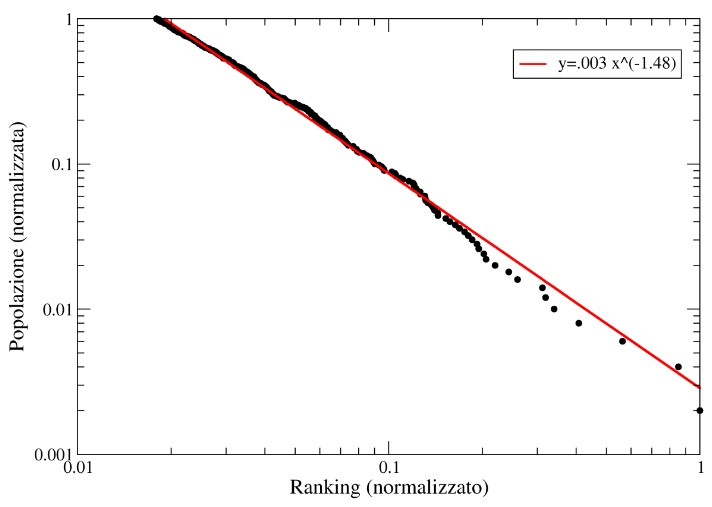
\includegraphics[scale=0.65]{cities_ranking.jpg}
\end{center}
This can be explained considering the fact that, storically, the population used to migrate towards the biggest cities of the country, because there were more job opportunities. Thus one can say that big cities have a preferential attatchment. \\ \\ 
Let $x$ be a random variable and $\{x_1,x_2, . . . , x_N\}$ a sample of experimental observations of the variable, ordered in such a way that $x_1 \geq x_2 \geq . \ . \ . \ \geq x_N$. \\ 
Then, the ranking distribution is created by assigning to the position $j$ in the order the corresponding value in the sampe, which is given by the map $x_j = f(j)$. Also, usually the elements are normalized like $y_j = x_j/x_1$. \\ 
By definition, $j/N$ is the frequency of the event $\{x \ | \ x \geq x_j \}$, that is, the probability that the variable $x$ has a value larger that $x_j$ for larger values of $j$. \\ \\
The cumulative distribution is defined as $F(x) = P\{u \ | \ u \leq x_j\}$, that is, the probability that the value $u$ is smaller that $x$. Of course, this probability is equal to the integral of the distribution in the range $[-\infty,x]$. \\
The relation between the frequency $j/N$ and the cumulative distribution is given by:
$$
	F(x_j) = 1 - \frac{j}{N} = 1 - \frac{J(x_j)}{N}
$$
where $J(x_j)$ is the inverse of the ranking, so it's the function that returns the position of a certain value of $x$ in the sample's order. \\
Since the cumulative distribution is the integral of the probability distribution, the latter can be obtained by differentiating the first:
$$
	p(x) = \frac{dF}{dx} \ \ \longrightarrow \ \ p(x) = -\frac{1}{N} \frac{dJ}{dx}
$$

\section{Laplace problem}
Let's suppose that we are tossing a coin, and the probability of gettin head is $p$ and the probability of getting tails is $1-p$. The event $E$ is $x_{n+1}$ outcome, and $H_n$ is $\{x_1,x_2,...\}$, so the first is the future and the second is the past. \\
Now we ask ourselves what is the probability that the next result of the toss is going to be heads:
$$
	p(x_{n+1}=H | H_n) 
$$
The most intuitive way to calculate this probability would be to use the frequentistic definition, so to count how many times we have gotten heads over the entire number of tries (we are considering the number of tries to be very big of course)
$$
	p = \frac{n_H}{N}
$$
Unfortunately, this is not the right way to do it. \\ \\
The probability of getting a given sequence of heads and tails is
$$
	p(\{x_k\}) = p^J(1-p)^{n-J}
$$
where $J$ is the number of times that we get heads. \\
Now if we integrate we get
$$
	\int_0^1 p^J(1-p)^{n-J}dp = \frac{J!(n-J)!}{(n+1)!}
$$
so
$$
	p(x_{n+1}=H|\{\}) = \frac{(n+1)!}{J!(n-J)!}p^J(1-p)^{n-J}
$$
which is a binomial distribution. \\
Now we calculate the average value of the probability
$$
\int_0^1 p\frac{(n+1)!}{J!(n-J)!}p^J(1-p)^{n-J}dp = \frac{J+1}{n+2}
$$
and we see that it isn't $J/n$, as one would have expected. 

\chapter{Basic models}
\section{Linear models}
The most simple model possible is the linear model
$$
	\dot{x} = Ax
$$
Albeit this model is easy, there are a few complications that have to be taken into account:
\begin{itemize}
	\item When the number of dimensions increases it becomes complicated. 
	\item If we consider the determinant
$$
	det(\la I - A) = 0
$$
we obtain a polinomial equation, that can be very hard to solve. 
	\item To further complicate things, $A$ might not be known, but we could have an ensemble of matrices. 
	\item The point $x=0$ is always a critical point, so we can always linearize the system around this point, but if $A$ has critical points then we get those as well. 
\end{itemize}
By solving the determinant equation, we get the eigenvalues $\la$, whose study can tell a lot about the behaviour of the solutions. \\
If $Re \la \leq 0$, this means that the exponential term of the solution shrinks, so it converges. \\ \\
Robustness means that if we perturb the system, the solutions don't change too much. A model must be robust, otherwise it can fit any kind of data simply by slightly changing the parameters. \\ \\
The formal way to write the solution of such a linear system is
$$
	x(t) = x_0\exp(At)
$$
For coefficients $\la^*$ such that $Re\la^* > 0$, we have that
$$
	|\delta x| \approx |e^{\la^* t}||\delta x_0|
$$
This is very tipical, and from this rises the chaos theory. In this case, even a small error in the initial condition will increase the error in the model exponentially fast. \\ \\
We get another interesting model by adding some noise to the linear model
$$
	\dot{x} = Ax + \xi(t)
$$
We consider a special solution of the form
$$
	x = e^{At}y
$$		
and we substitute in the equation
$$
	\dot{x} = A\exp(At)y + \xi(t) = A\exp(At)y + \exp(At)\dot{y}
$$	
$$
	\dot(y) = \exp(-At)\xi(t)
$$
So the complete solution of the problem is
$$
	x(t) = \exp(At)x_0 + \int_0^t \exp(A(t-s))\xi(s)ds
$$
If the system is stable (negative real part of lambda) and we use a periodic forcing, the solution is still a periodic function with different period. \\ \\
Now we want to consider the case of a perturbed matrix:
$$
	\dot{x} = (A+\varepsilon B)x
$$
with $\varepsilon \ll 1$. \\
The solution is
$$
	x(t) = \exp((A+\varepsilon B) t)x_0
$$
and to understand the system's sensitivity we calculate the derivative for small perturbations
$$
	\frac{d}{d\varepsilon}\exp((A+\varepsilon B)t)
$$
but the problem is that usually the two matrices are not commutative. \\
If we take the special solution $x = \exp(At)x_0$ and we substitute we get
$$
	\dot{y} = \varepsilon\exp(-At)B\exp(At)y
$$
and, if $A$ and $B$ do not commute, this equation is very difficult to solve. \\
An approximate solution is
$$
	y(t) = y_0 + \varepsilon\int_0^t \exp(-As)B\exp(As)y_0ds + O(\varepsilon^2)
$$
and the solution for x is
$$
	x(t) = \exp(At)x_0 + \varepsilon\int_0^t \exp(A(t-s))B\exp(As)x_0ds + O(\varepsilon^2)
$$
Now, the sensitivity of the system is
$$
	\frac{dx}{d\varepsilon} = \int_0^t \exp(A(t-s))B\exp(As)x_0ds 
$$
In the particular case where the matrix is diagonal, the sensitivity becomes
$$
	\frac{dx}{d\varepsilon} = \int_0^t \exp(\la_i(t-s))B_{ij}\exp(\la_js)x_0ds 
$$

\section{The neuron model}
In this model we have two variables, $x$ and $w$, and two differential equations to describe their dynamics
$$
	\dot{x} = x - \frac{x^3}{3} - w + I(t)
$$
$$
	\dot{w} = \frac{1}{\mu}(x+a-bw)
$$
This system is of course not linear, because we have a cubic term in the dynamics of $x$. \\
We require $\mu$ to be big, so that $w$ is the slow variable, whereas $x$ is the fast variable. \\
The fact that the two variables have different growth speeds is quite important, because it allows us to study them separately, and this reduces the complexity of the system. \\
The difference in the speed of the variables makes the system stiff, which means that it's very hard to integrate numberically. \\ \\
The key to studying this system is in the nullcline. We find the two nullclines by putting the two derivatives equal to zero, so one is a straight line and the other one is a cubic. \\
The two nullclines intersect, and the point where they intersect is the equilibrium point of the system. Furthermore, the cubic nullcline has two critical points. Since $x$ is the fast variable, the point follows the cubic nullcline in its dynamics. Once it reaches one of the two critical points, during its motion, it jumps to the other branch of the nullcline. So in the end one gets a periodic motion. \\ \\
Suppose now that $I(t)$ is of the form
$$
	I(t) = I_0 + \Delta I \delta(t)
$$	
so we give an impulse to the point. \\
What happens now is that, if $\Delta I$ is small, the point oscillates briefly around the critical point and falls back into it, but if the the impulse is big, the point excapes and makes a very big oscillation. \\
In this system we have an Hopf bifurcation. \\

We can take many neurons and link them one-to-one in a circular graph. Each neuron is going to have its own system of differential equations of the Fitzhugh-Nagumo model. Now, since the neurons are linked, the firing of a neuron stimulates the following one, so they interact.
$$
	\dot{x_k} = F(x_k) + \varepsilon(x_{k-1}-x_p)
$$
Does exist a critical value of $\varepsilon$ so that the system auto-fuels and mantains its motion indefinitely without and external source?

\subsection{Hopf Bifurcation}
Sometimes the orbits of a dynamical system converge not in a single point but in limit circle near the stable point.
This is called \emph{Hopf Bifurcation}.
That type of phenomena is recurrent in nature: one example may be the Ising's model in which the system passes from a one stable point state to a two stable points state with a phase transition.
In that specific case we observe a bifurcation of the system's free energy.\\
We have to see the Hopf bifurcation as a new dynamical state that has a periodic orbit as a solution.
However, it's important to observe that a Hopf bifurcation is not an equilibrium state for the system.\\
For example, consider a circular network of identical neurons characterized by a function $\dot{x}_k$.
The dynamic is described by a simple law
$$
    \dot{x}_k=F(x_k)+\epsilon x_{k-1}
$$
in which the function F() is taken from the Fitzhug-Nagumo model and the other term represents the system dynamic.\\
If $x_P$ is an equilibrium point for all neurons then we can verify that exists an $\epsilon=\epsilon_C$ that produces a non-trivial solution.
In particular, with that value of $\epsilon$ we can create a stationary periodic state with a periodic signal (moving wave): that's a self-solution for the system.
Obviously, this example do not conserve the total energy of the system.

\chapter{Dynamical Systems}
% chaotic dynamics
A dynamical system is given by a space $M \subseteq R^d$ endowed with a collection of maps $\phi^t:M\rightarrow M$, where $t \in R$ and where $M$ is the phase space, with the "group property":
$$
	\phi^{t+s} = \phi^t o \phi^s
$$
The maps $\phi^t$ are usually called flows. \\ 
This formalization works for systems whose equations don't depend explicitly on time. \\
A typical example of a dynamical system is that of the solutions of a differential equation. So if we have a differential equation
$$
	\dot{x} = f(x)
$$
with initial condition $x(0) = x_0$, the flow is the function that takes the initial condition and returns the correct solution for the differential equation. So if this ODE has a global solution, so a solution $x(t)$ that satisfies the initial condition, then 
$$
	\phi^t(x_0) = x(t)
$$
We must also assume the uniqueness of the solution, that is, for one initial condition we only have one solution. //
Non-autonomous ODEs, where the equation field depends on time
$$
	\dot{x} = f(x,t)
$$
can be converted into autonomous ODEs in higher dimensions, going back to the previous simpler case. \\
We consider $\overline{M} = M \times R$ with $y = (x,t) \in \overline{M}$, and we define
$$
	F(x,t) = (f(x,t),1)
$$
with $f : M \times R \rightarrow R^d$ and $F : M \times R = \overline{M} \rightarrow R^{d+1}$. At this point we can write the new differential equation:
$$
	\dot{y} = F(y)
$$
with initial condition $y(0) = (x_0,0)$. For this to be useful, we must show that knowing the solution to this new equation implies knowing the solution for the original one. \\
Say $y(t) = (x(s),t(s))$ is a solution for the new equation
$$
	\begin{patrix}
		\dot{x}(s) \\ 
		\dot{t}(s)
	\end{patrix} = 
	F
	\begin{patrix}
		x(s) \\ 
		t(s)
	\end{patrix} =
	\begin{patrix}
		f(x(s),t(s)) \\ 
		1
	\end{patrix} = 
$$
$$
	\dot{x} = f(x,s) \ \ \ \ \ \dot{t} = 1
$$
with initial conditions $x(0) = x_0$ and $t(0) = 0$. For what concerns t, it's the identity function, so $t(s) = s$, which means that I can invert $t$ and $s$, so going back to the first equation we have
$$
	\dot{x} = f(x,t)
$$
which was our original equation. This means that a solution for the non autonomous equation is also a solution to the new autonomous one. \\
So, if we have a theory that treats non autonomous systems, that theory must also be able to treat autonomous systems. \\ \\
If the $t$ variable is a natural number, we call it $n$
$$
	\phi^n = T^n
$$

% dynamical systems with discrete time
% malthus
$$
	x_{n+1} = \alpha x_n
$$
where $x_n$ represents the population in year $n$. For $\alpha > 1$, we have population growth and for $\alpha < 1$ the population decreases. \\
If at time $t=0$ the population is $x_0$, at a given time we have
$$
	x_n = T_n(x_0) = \alpha^n x_0
$$
% velhurst
This model takes into account the fact that the higher the population is, the more resouces are needed, so there should be a limit that can't be surpassed, because the enviroment wouldn't be able to sustain it
$$
	x_{n+1} = \alpha x_n(A-x_n)
$$
Now we change variable, defining $\hat{x} = x/A$, and we get
$$
	\frac{x_{n+1}}{A} = A\alpha \frac{x_n}{A}\left(1 - \frac{x_n}{A}\right)
$$
$$
	\hat{x_{n+1}} = r \hat{x_n}(1-\hat{x_n})
$$
which is the logistic map:
$$
	T(x) = rx(1-x)
$$
We take $x$ between $0$ and $1$ and $r$ between $0$ and $4$. The graph is a parabola upside down.

\section{Malthus model}
Let's take the expression
$$
	x_{n+1} = \alpha x_n
$$
where $x_n$ represents the population in year $n$. For $\alpha > 1$, we have population growth and for $\alpha < 1$ the population decreases. \\
If at time $t=0$ the population is $x_0$, at a given time we have
$$
	x_n = T_n(x_0) = \alpha^n x_0
$$
\section{Velhurst model}
This model takes into account the fact that the higher the population is, the more resources are needed, so there should be a limit that can't be surpassed, because the environment wouldn't be able to sustain it
$$
	x_{n+1} = \alpha x_n(A-x_n)
$$
Now we change variable, defining $\hat{x} = x/A$, and we get
$$
	\frac{x_{n+1}}{A} = A\alpha \frac{x_n}{A}\left(1 - \frac{x_n}{A}\right)
$$
$$
	\hat{x_{n+1}} = r \hat{x_n}(1-\hat{x_n})
$$
which is the logistic map:
$$
	T(x) = rx(1-x)
$$
We take $x$ between $0$ and $1$ and $r$ between $0$ and $4$. The graph is a parabola upside down.

\end{document}
